\chapter{Realisation}
\section*{Introduction}
In this chapter, we describe the working environment used during
the realization of our application. We will also describe its layout
physical using a deployment diagram. Then, we
detail the work carried out and the results obtained using a set
of screenshots representing the interfaces of the different functionalities of
our app.
\section{Technical specification}
In this section, we will present the technical choices relating to
the hardware and software environment that contributed to the realization of our
application.
\subsection{Hardware environment}
During the different stages of our project, i.e. documentation,
code implementation and testing, we had:
\begin{itemize}
\item A personal computer with the following configuration:
\begin{itemize}
\item Brand: Lenovo;
\item Processor: AMD Ryzen 3 3200U with Radeon Vega Mobile Gfx 2.60 GHz ;
\item RAM: 12 GB;
\item Hard disk: 1TB;
\item System type: Windows 64-bit operating system.
\end{itemize} 
\item A Smartphone with the following characteristics:
\begin{itemize}
\item Brand: Itel;
\item RAM: 1 GB;
\item Processor: Quad Core Qualcomm Snapdragon 810 @ 2.3GHz;
\item System version: Android 9.0;
\end{itemize}
\end{itemize}
\subsection{Software environment}
Throughout the development phase, we used the tools
software and the following development languages:
\subsubsection{Software tools}
During the implementation of our project we used the following software :
\paragraph*{Android Studio}
Android Studio is an integrated development environment for android, IOS, web, and Windows platforms. Developers use this environment
to develop Cross platforms applications. Android Studio allows
mainly editing the Dart files and configuration files of the application.
\begin{figure}[H]%
    \center   
    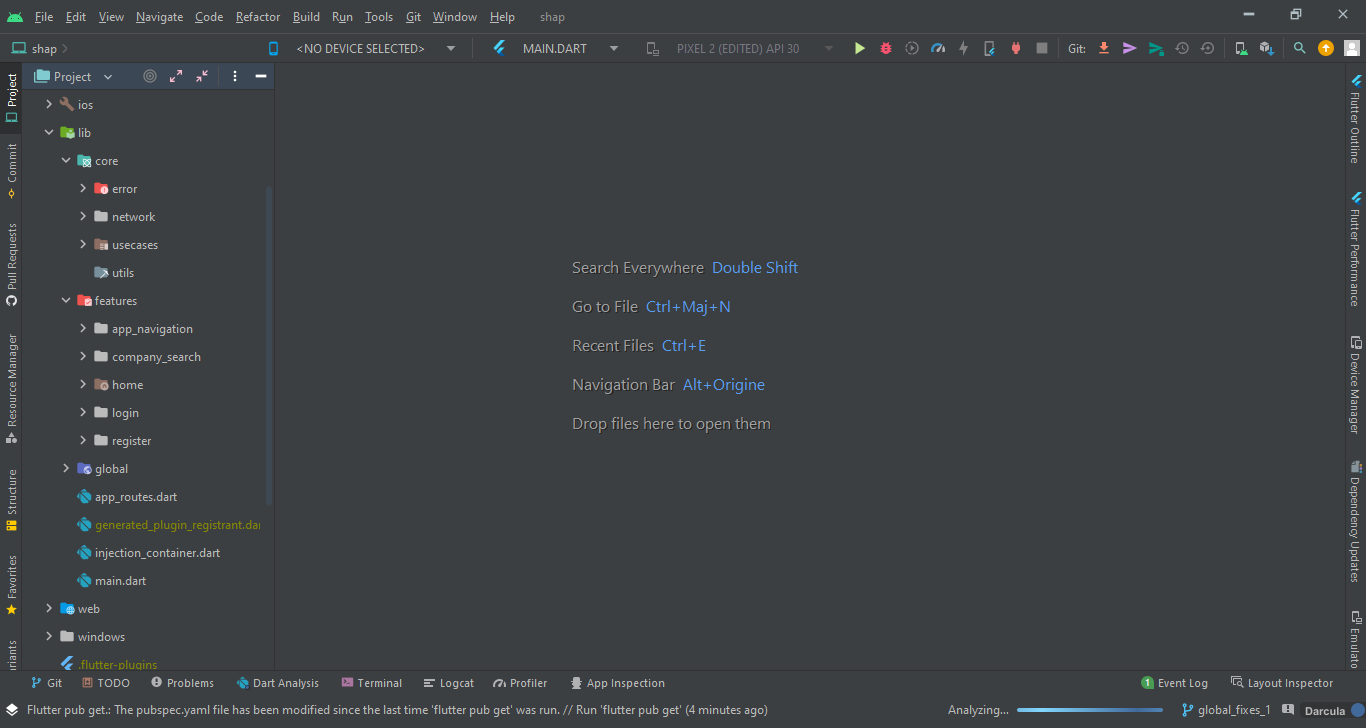
\includegraphics[scale=0.5]{as.png}
    \caption{Android Studio}
\end{figure}
\paragraph*{PostMan}
Postman is an API platform for developers to design, build, test, and iterate their APIs. As of April 2022, Postman reports having more than 20 million registered users and 75,000 open APIs, which it says constitutes the world's largest public API hub.\\
In our application, we used PostMan to test APIs.
\begin{figure}[H]%
    \center   
    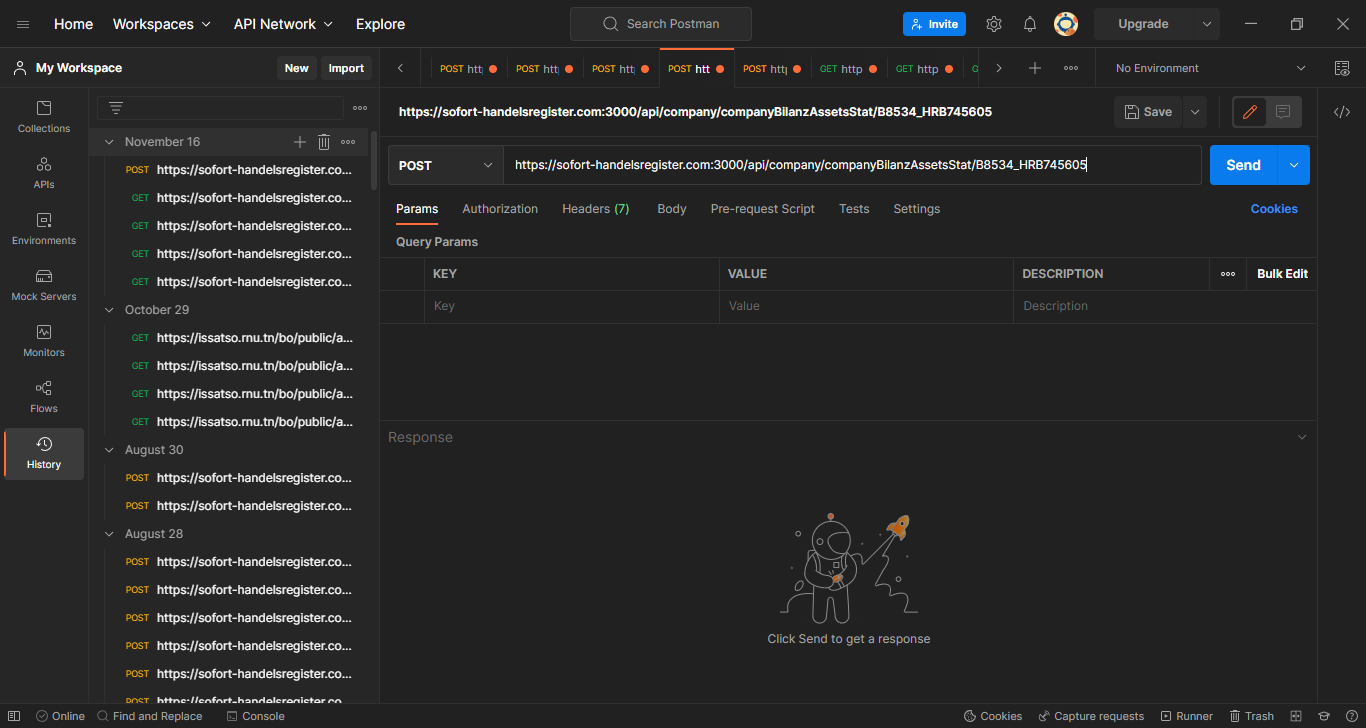
\includegraphics[scale=0.5]{pm.png}
    \caption{PostMan}
\end{figure}
\paragraph*{StarUML}
StarUML is a software engineering tool for system modeling using the Unified Modeling Language, as well as Systems Modeling Language, and classical modeling notations. It is published by MKLabs and is available on Windows, Linux, and macOS. Wikipedia.\\
In our application, we used StarUML to establish UML diagrams for this report.
\begin{figure}[H]%
    \center   
    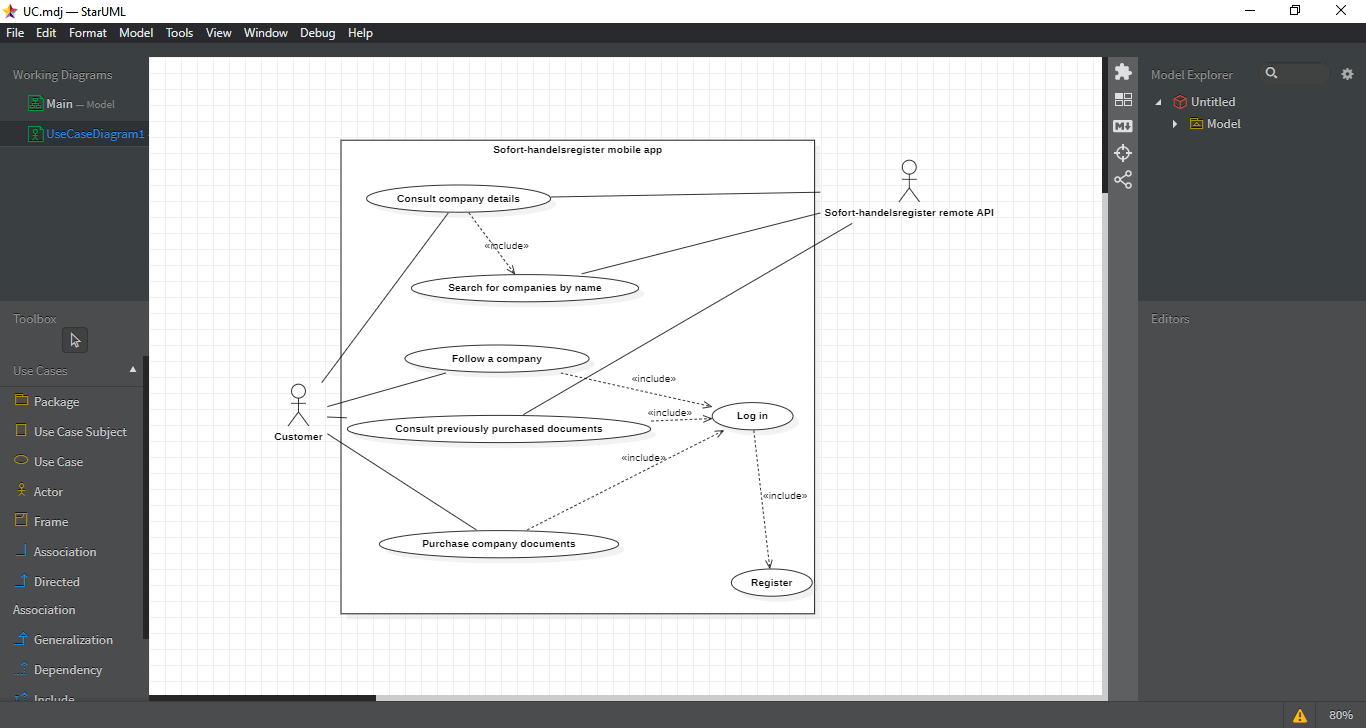
\includegraphics[scale=0.5]{star.png}
    \caption{PostMan}
\end{figure}
\paragraph*{Social media login providers}
The following online platforms were used in our application to provide and configure the login process using social media accounts within our application those platforms are respectively Google Cloud, Meta for developers, LinkedIn for developers, and xing for developers as shown in the following figures.
\begin{figure}[H]%
    \center   
    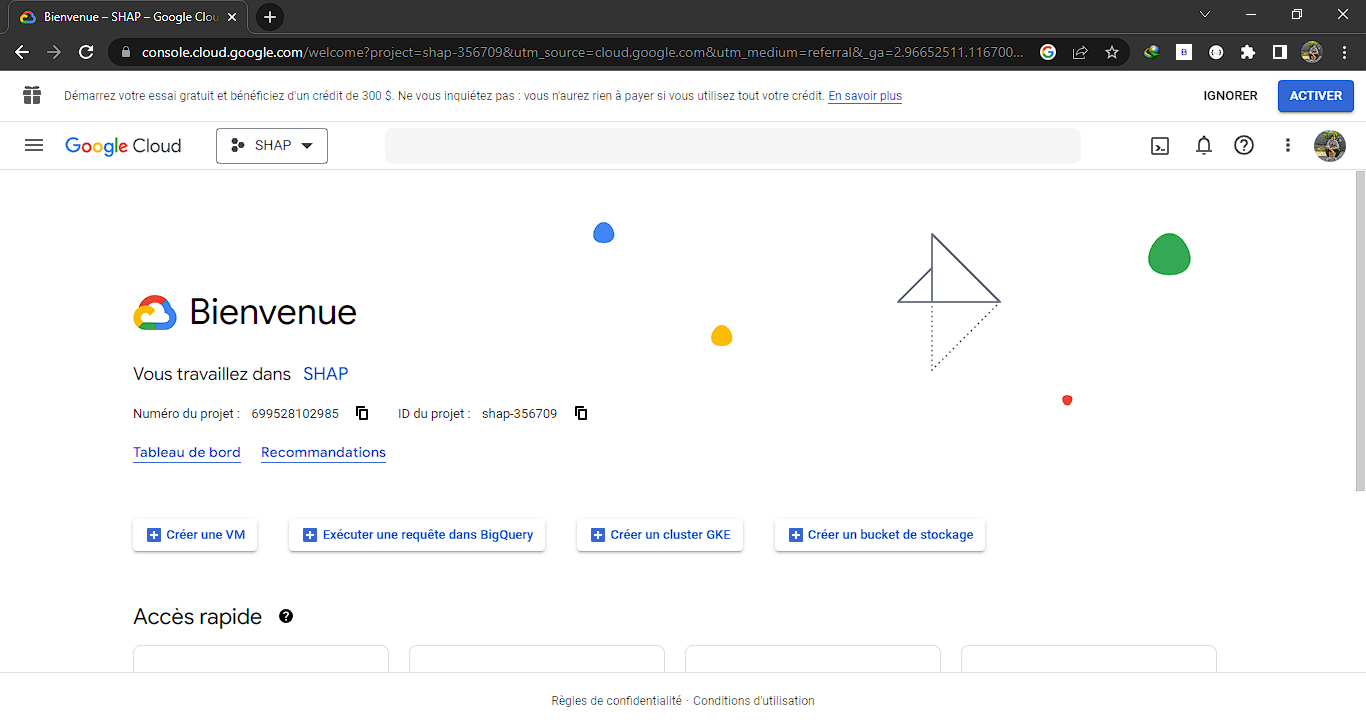
\includegraphics[scale=0.5]{google.png}
    \caption{Google cloud}
\end{figure}
\begin{figure}[H]%
    \center   
    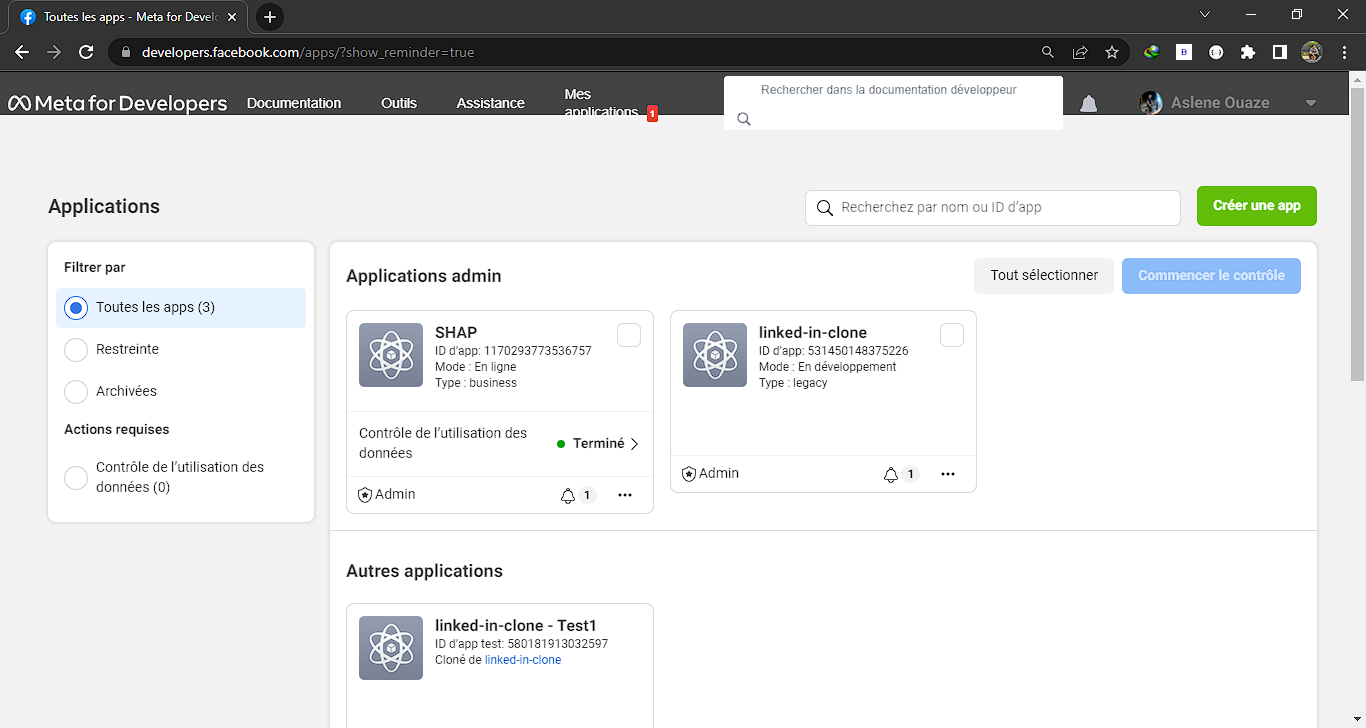
\includegraphics[scale=0.5]{meta.png}
    \caption{Meta for developers}
\end{figure}
\begin{figure}[H]%
    \center   
    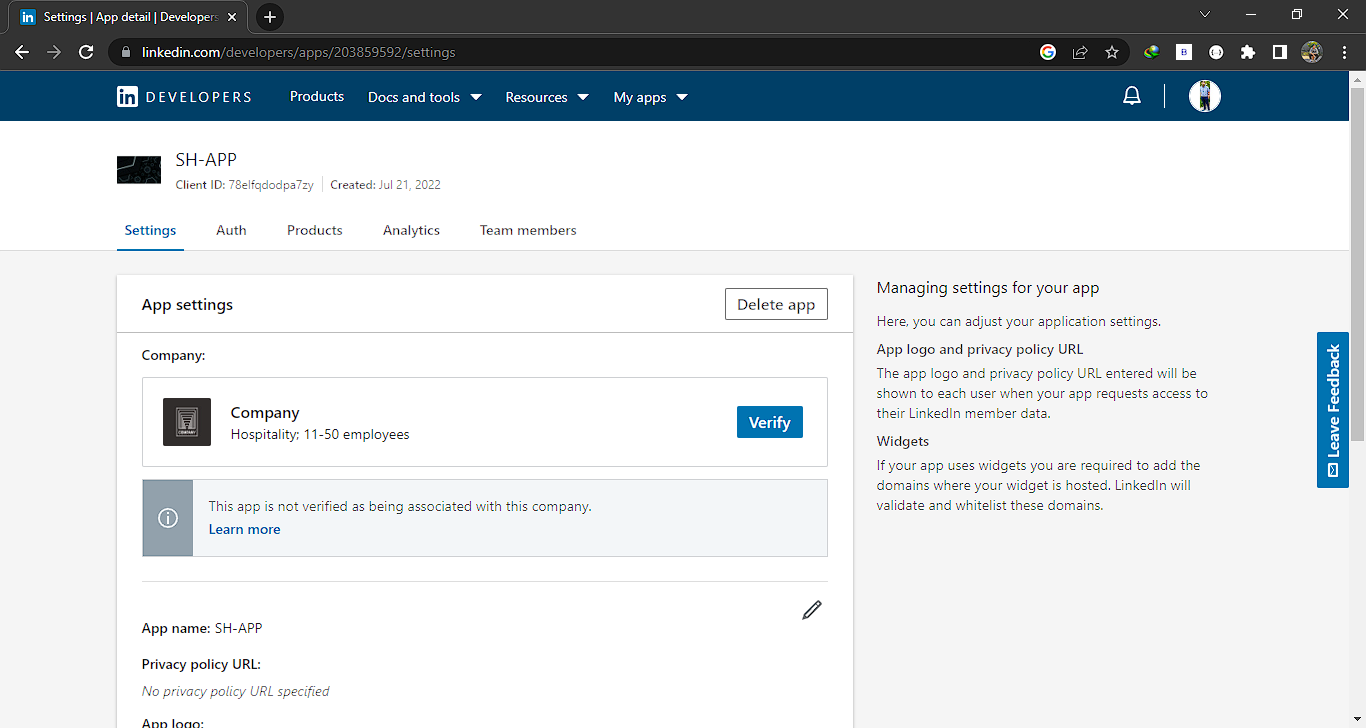
\includegraphics[scale=0.5]{linkedin.png}
    \caption{LinkedIn for developers}
\end{figure}
\begin{figure}[H]%
    \center   
    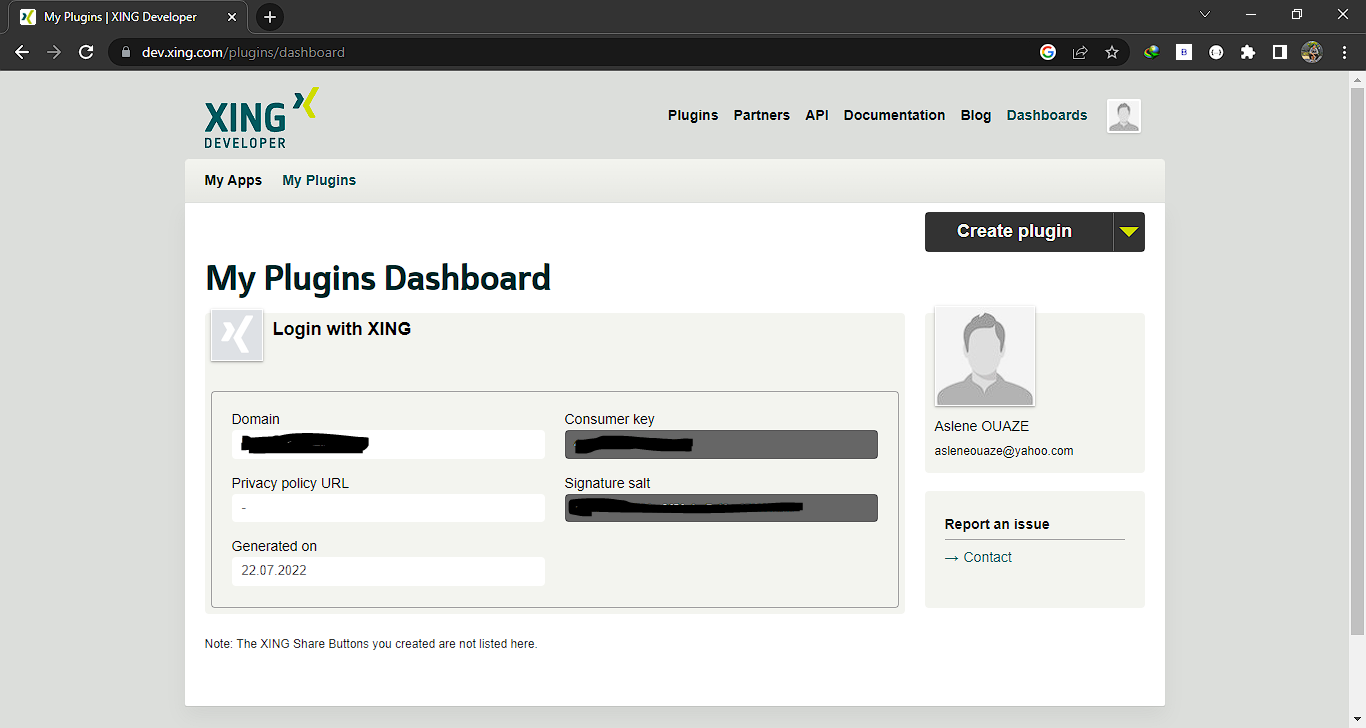
\includegraphics[scale=0.5]{xing.png}
    \caption{Xing for developers}
\end{figure}
\subsubsection{APIs and libraries}
\paragraph*{Sofort-handelsregister API}
The Sofort-Handelsregister API is an API developed by the host company Glocal IT, its currently used in the web platform \href{https://sofort-handelsregister.com/}{Sofort-handelsregister. com}that offers similar services to our applications, the API allows us to communicate with the Glocal It database that contains company data, statistics, documents, and customer information as well as a robust login and register service for customers.\\
We can integrate it into mobile or web applications regardless of the programming language used.
\paragraph*{Libraries}
\begin{table}[H]
\begin{tabular}{|l|l|}
\hline
\textbf{Library}        & \textbf{Usage}                                                                                                                                                                                           \\ \hline
flutter\_facebook\_auth & \begin{tabular}[c]{@{}l@{}}Add Facebook login to our flutter app. \\ Feature includes getting user information, profile picture, and more. \\ This plugin also supports Web and macOS.\end{tabular}       \\ \hline
linkedin\_login         & \begin{tabular}[c]{@{}l@{}}Library for login with LinkedIn OAuth V2 service.\\ This library helps to implement authorization with LinkedIn OAuth API's.\end{tabular}                                     \\ \hline
google\_sign\_in        & \begin{tabular}[c]{@{}l@{}}Flutter plugin for Google Sign-In, \\ a secure authentication system for signing in \\ with a Google account on Android and iOS.\end{tabular}                                 \\ \hline
webview\_flutter\_plus  & \begin{tabular}[c]{@{}l@{}}An extension of webview\_flutter to load local HTML,CSS\\  and Javascript from Assets or Strings and much more.\end{tabular}                                                  \\ \hline
flutter\_bloc           & \begin{tabular}[c]{@{}l@{}}Flutter Widgets that make it easy to \\ implement the BLoC (Business Logic Component) design pattern.\\ Built to be used with the bloc state management package.\end{tabular} \\ \hline
email\_validator        & A dart class for validating email addresses                                                                                                                                                              \\ \hline
shared\_preferences     & \begin{tabular}[c]{@{}l@{}}Flutter plugin for reading \\ and writing simple key-value pairs (local cache). \\ Wraps NSUserDefaults on iOS and SharedPreferences on Android.\end{tabular}                 \\ \hline
connectivity\_plus      & \begin{tabular}[c]{@{}l@{}}Flutter plugin for discovering the state of the network \\ (WiFi \& mobile/cellular) connectivity on Android and iOS.\end{tabular}                                            \\ \hline
\end{tabular}
\caption{Libraries}
\end{table}
\subsubsection{Programming languages}
\paragraph*{Dart}
Dart is a programming language designed for client development, such as for the web and mobile apps. It is developed by Google and can also be used to build server and desktop applications. It is an object-oriented, class-based, garbage-collected language with C-style syntax.
\paragraph*{XML}
The XML (Extensible Markup Language) allows the developer to create information formats
and share them via networks. This standard is used to describe data.
\paragraph*{JSON}
JSON(JavaScript Object Notation) is a lightweight data-interchange format that is easy to read and write and
frequently used by developers.
\subsection{Deployment diagram of the application}
The deployment diagram models the physical architecture of a system.
This diagram shows the topology of the software elements that are deployed over the material elements.
The following figure represents the deployment diagram of our application.
\begin{figure}[H]%
    \center   
    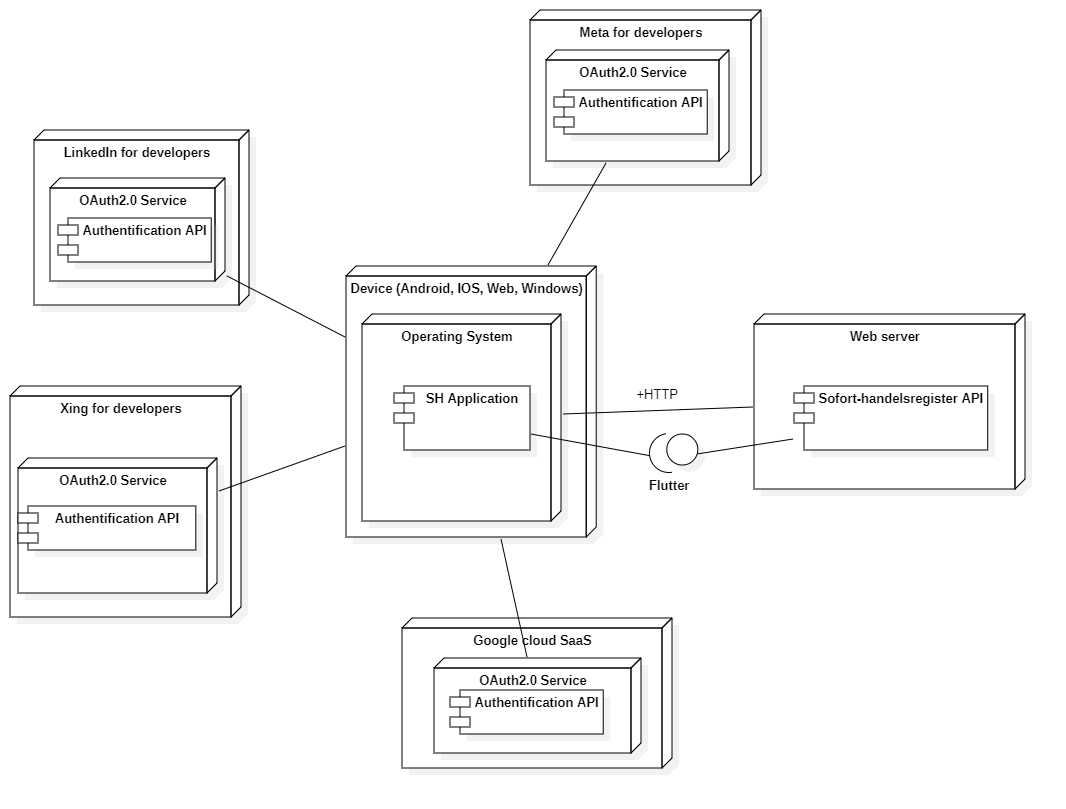
\includegraphics[scale=0.5]{deploy.png}
    \caption{Deployment diagram of the application}
\end{figure}
\section{Apllication interfaces}
In this part, we present the different functionalities of our
application by presenting the graphical interfaces produced:
\subsection{Launching the application}
The following figure represents the landing page of the application where the user can choose between two options login and searching for a company when choosing login the user will be redirected to the login interface, when choosing company search the user will be redirected to the company search interface 
\begin{figure}[H]%
    \center   
    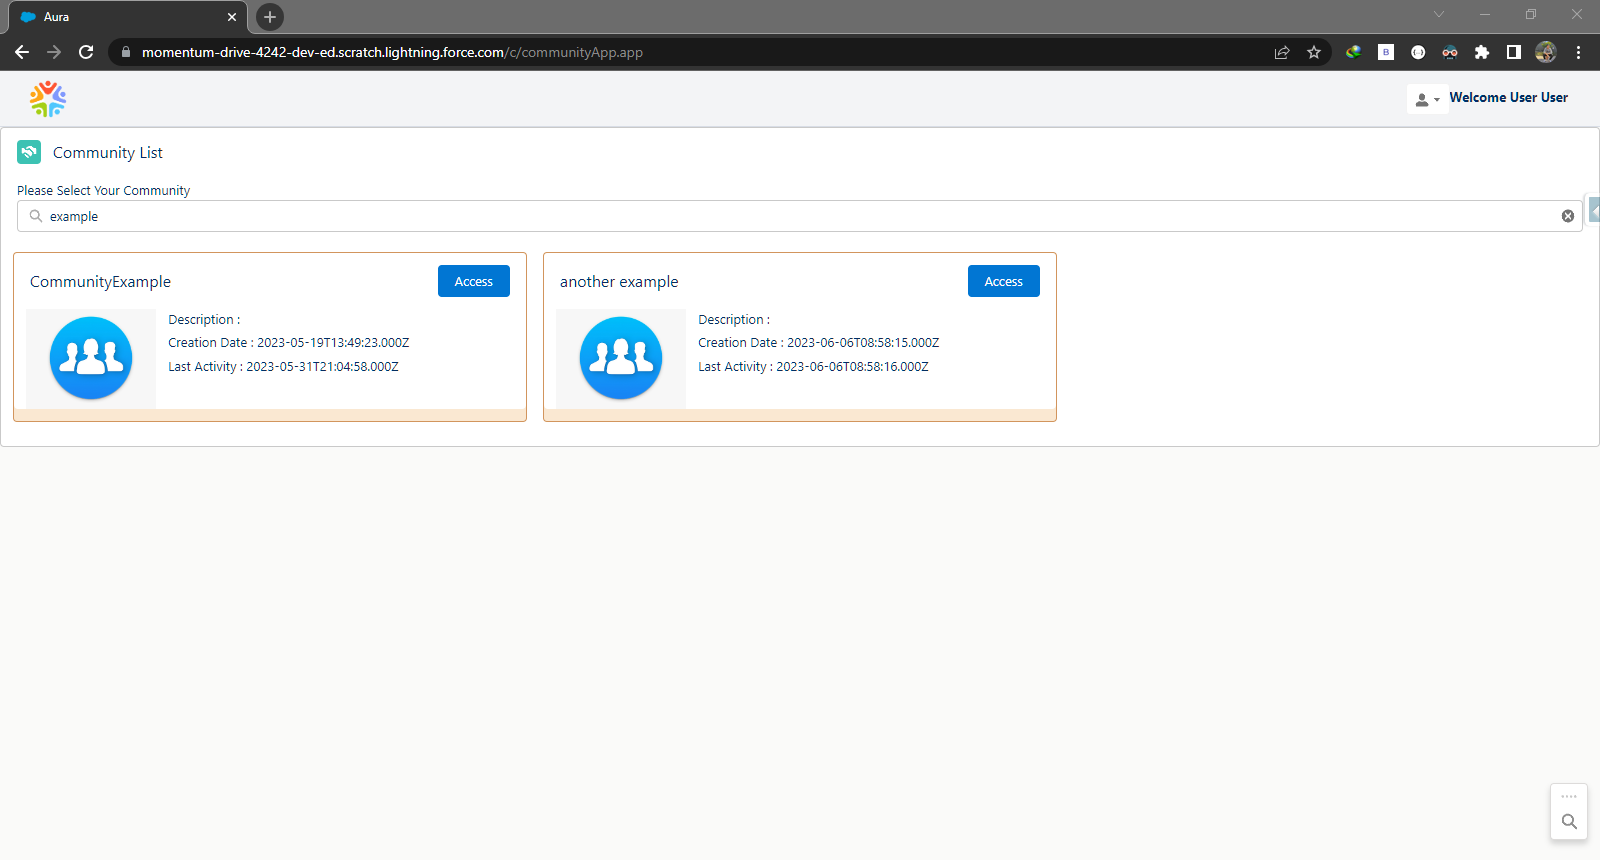
\includegraphics[scale=0.4]{home.png}
    \caption{Landing page of the application}
\end{figure}
\subsection{Authentication}
The following figure explains the authentification process. The user can input his account email and password, he can also tap the forgot password option to receive an email containing a link to set up his new password.
The buttons "Facebook", "Google", and "LinkedIn" can be used to log in using social media accounts.
\begin{figure}[H]%
    \center   
    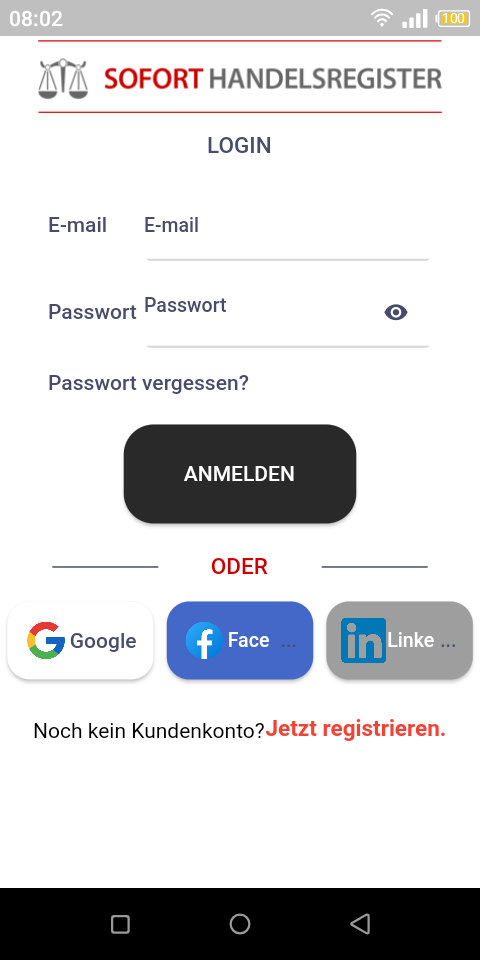
\includegraphics[scale=0.4]{login.png}
    \caption{Authentication page of the application}
\end{figure}
\subsection{Registeration}
The register interface contains the input fields: FirstName, LastName, Email, Password, Password confirm, and the accept terms and conditions check box that is necessary for a successful registration. Upon validating the form the user will be redirected to the login interface. 
\begin{figure}[H]%
    \center   
    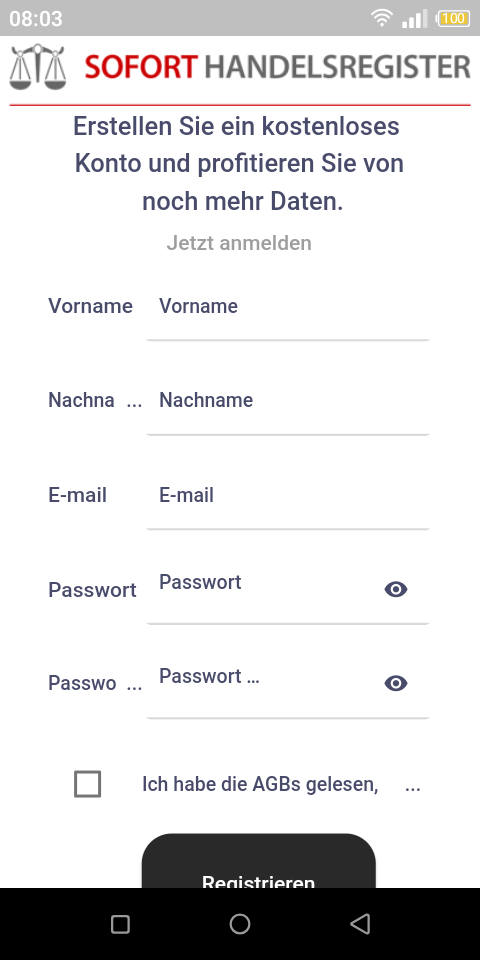
\includegraphics[scale=0.4]{register.png}
    \caption{Registeration page of the application}
\end{figure}
\subsection{Company search}
The following figure represents the company search interface where the user can input the full name of his wanted company or the first letter of it using the text input field on the top of the page. The search results are presented as an interactive list showing the name of the company, its full address, its current status, and its legal form.  
\begin{figure}[H]%
    \center   
    
    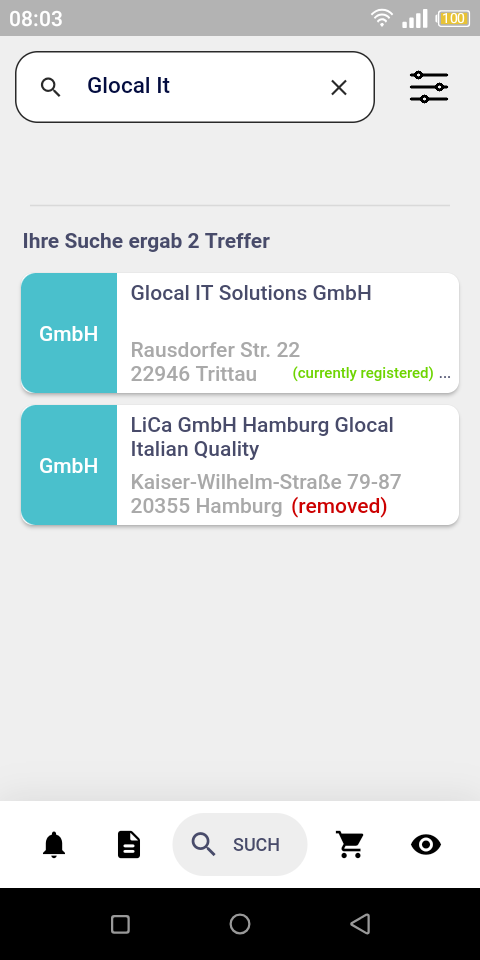
\includegraphics[scale=0.4]{search2.png}
    \caption{Company search page of the application}
\end{figure}
\subsection{Results filtering}
The filter interface allows the user to filter his search results using state, zip code, legal form, capital, and branch as shown in the following figure.
\begin{figure}[H]%
    \center   
    
    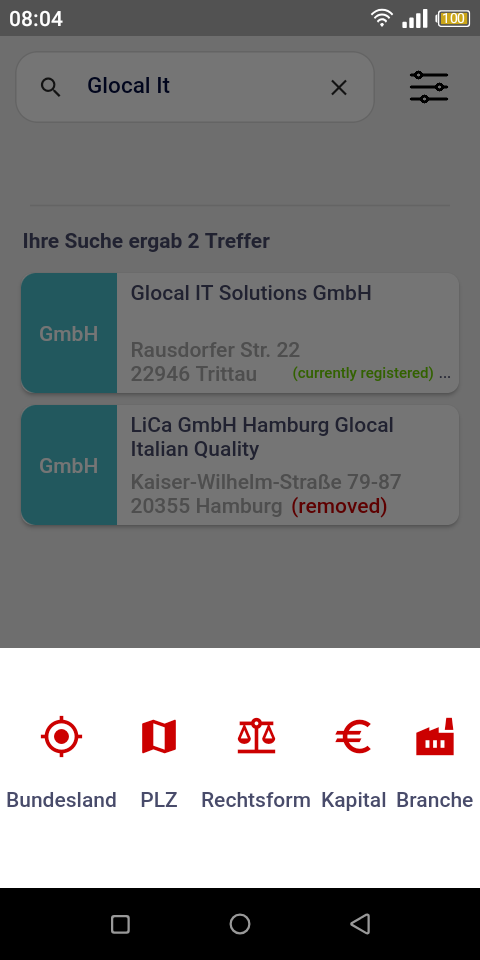
\includegraphics[scale=0.4]{filter1.png}
    \caption{Filter interface of the application}
\end{figure}
The filter interface presents two main types of filtering the first one represents the custom filter where the user can type the filter in the text input field as shown in the following figure.
\begin{figure}[H]%
    \center   
    
    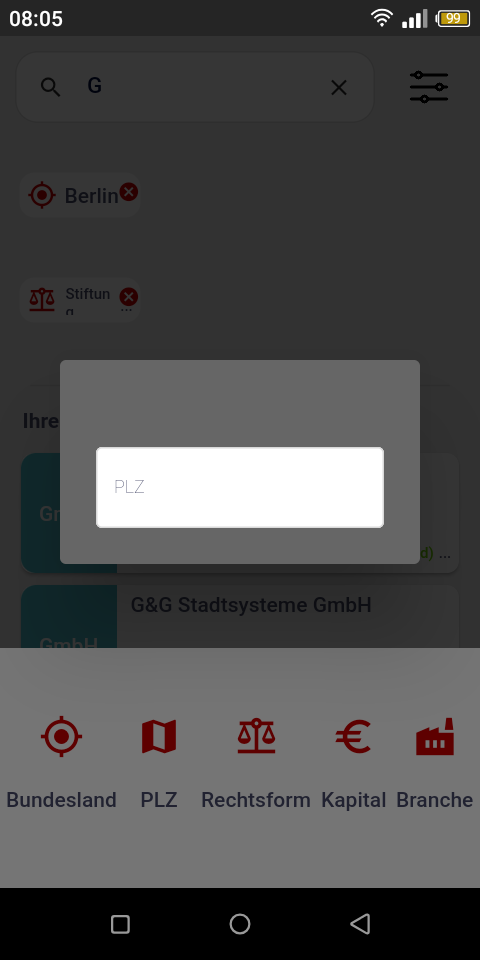
\includegraphics[scale=0.4]{filter3.png}
    \caption{Custom filter interface of the application}
\end{figure}
The second filter type represents the predefined options filter where the user can choose one or many pre-defined options as shown n the following figure.
\begin{figure}[H]%
    \center   
    
    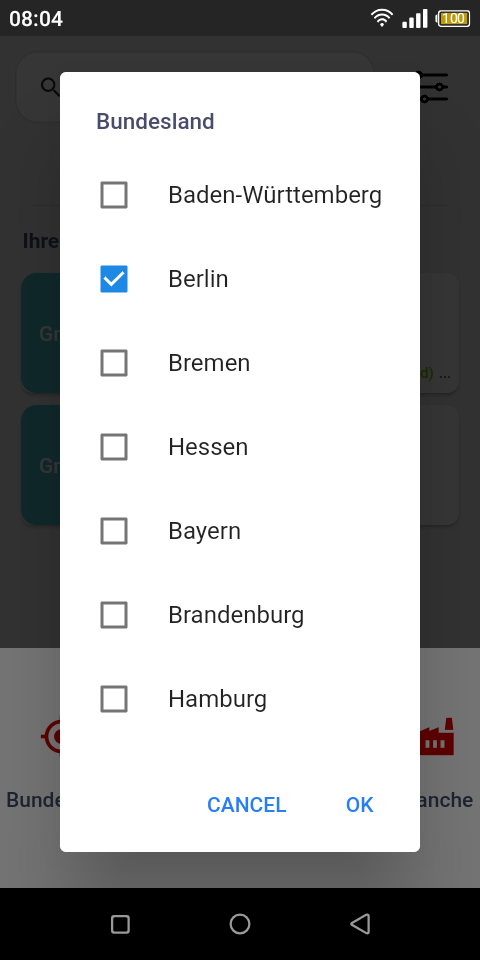
\includegraphics[scale=0.4]{filter2.png}
    \caption{Pre-defined filter interface of the application}
\end{figure}
After choosing all his filters the user may come back to his check his filtered results where he may find his applied filters displayed as shown in the following figure.
  \begin{figure}[H]%
    \center   
    
    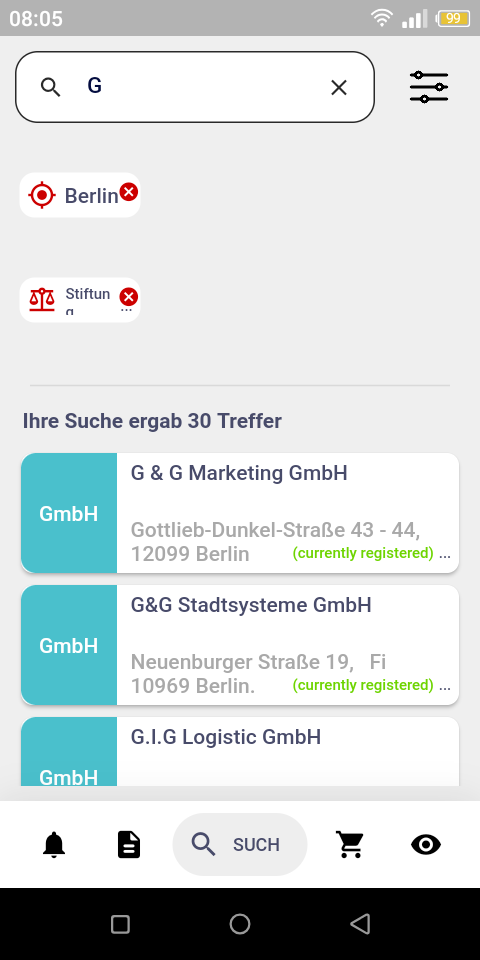
\includegraphics[scale=0.4]{search3.png}
    \caption{Filtered search results interface of the application}
\end{figure}
\subsection{Company Details}
After choosing an element from the list of results, the customer will be redirected to the company details interface where he may consult the company name, address, current status, legal form, officers, branch, phone, mobile phone, email, and website as shown in the following figure.
 \begin{figure}[H]%
    \center   
    
    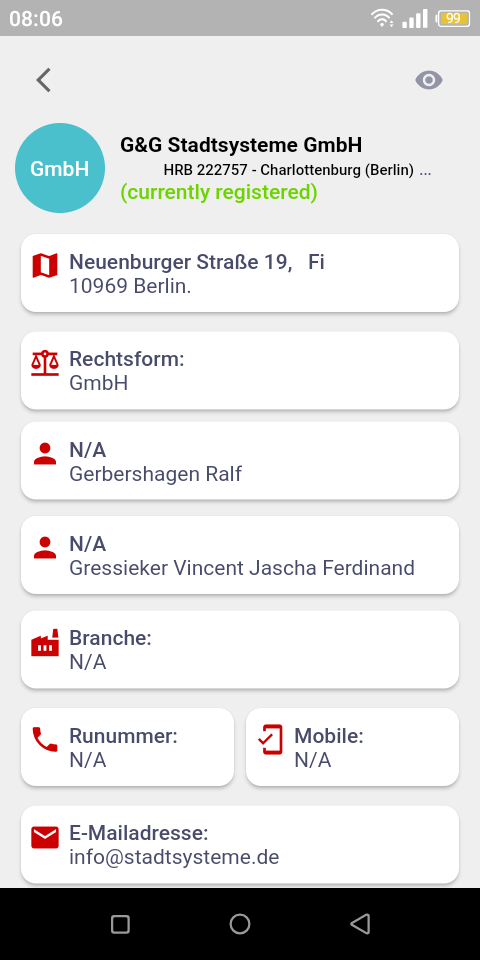
\includegraphics[scale=0.4]{details1.png}
    \caption{Company details interface of the application}
\end{figure}
The same interface presents the documents section where the list of documents is displayed and can be selected by the user to be added to the shopping cart using the toggle button in front of each element as shown in the following figure.
\begin{figure}[H]%
    \center   
    
    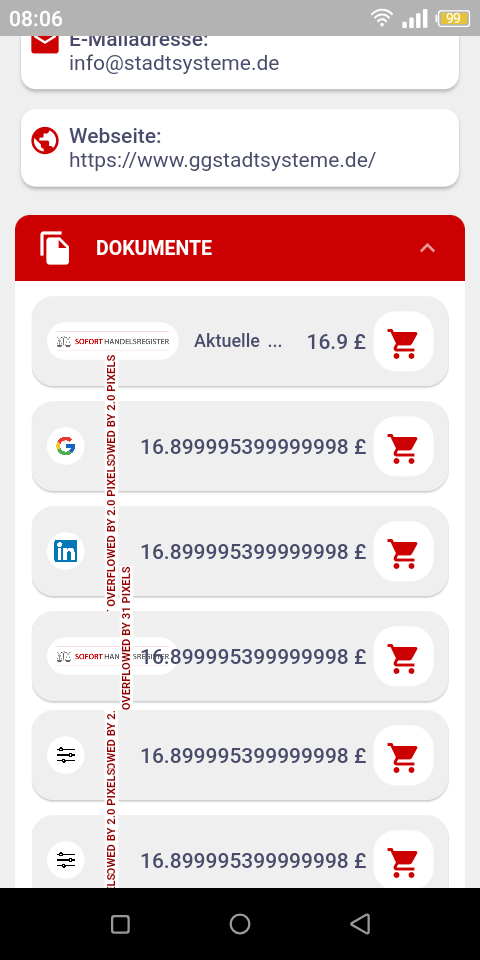
\includegraphics[scale=0.4]{details2.png}
    \caption{Document section interface of the application}
\end{figure}
The last part of the company details interface presents the notices section, insolvency check section, and statistics section available for free for the customer as shown in the following figure.
\begin{figure}[H]%
    \center   
    
    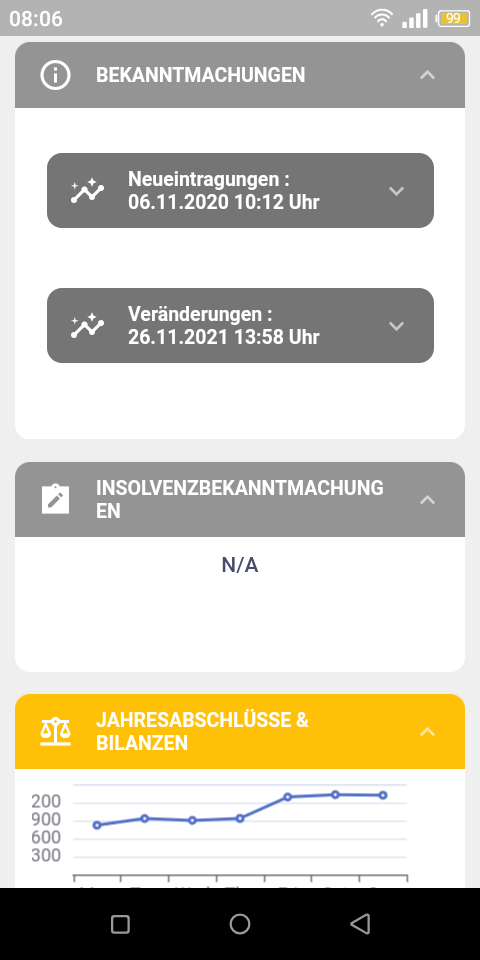
\includegraphics[scale=0.4]{details3.png}
    \caption{Extra section interface of the application}
\end{figure}
\section*{Conclusion}
In this chapter, we presented the technical specification of our
application through the introduction of hardware and software environments. Ultimately,
we have described the functionalities of our application,
illustrated by screenshots of its user interfaces.
We end our report with the general conclusion and the different
prospects.